

	\subsection{Pesos de los eventos}

	Considerando los algoritmos en las secciones \ref{peso_hexagonos} y \ref{rayleigh}

		
		Para solucionar el desfase entre los pesos que obtengo mediante la hora local y la ascensión recta, lo que hice fue poner adrede un valor de desfase cuando calculo el valor $h$, le agregue $2\,$hr. 

\subsection{Acerca del algoritmo}

	%Contexto: Yo quiero hacer el análisis de los pesos de los hexágonos para distintas frecuencias, por lo que esperaría que para cada frecuencia a analizar se utilice el mismo algoritmo para todos.

	% Mi duda: En el código del paper 18, el algoritmo hace distinción entre la frecuencia sidérea y las demás. Comparando ambos algoritmos, como se muestra en la Fig.\,\ref{fig:alter_24}, se ve que ambos dan un resultado similar para los pesos de los hexágonos a menos de un desfase de $75^o$ o $5\,$hrs sidéreas. Los gráficos de esta figura se hicieron con el mismo data set.

	Otra cosa que me resultó curiosa fue que usando $N=360$, tengo problemas con la frecuencia solar, donde aparecen 0 cada 5 min, coincide con el rate de actualización del archivo de weather. Así usando este bineado, aparece ese problema, recomendaría no trabajar con bines de $1^o$ en ascensión recta.
	\begin{figure}[H]
	\centering
	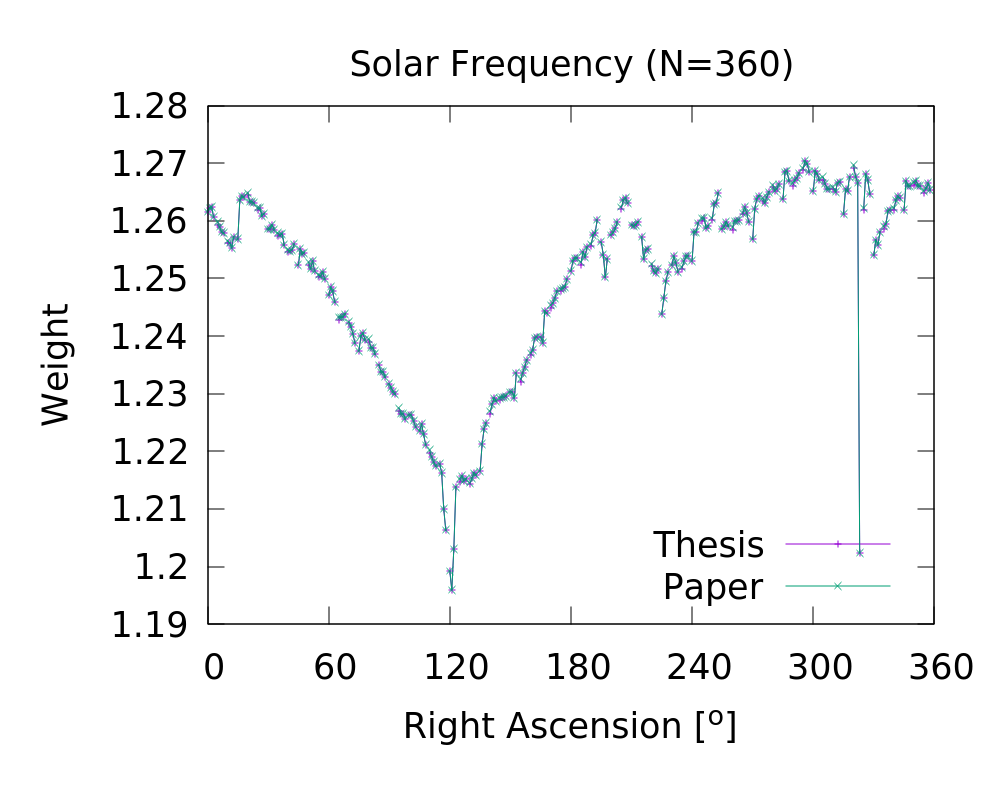
\includegraphics[width=\linewidth]{Graficos/solar_my_and_paper_in_360_2.png}
	\caption{Usando 360 bines, nótese que la media es distinta a la figura anterior.}
	\label{fig:solar_360}
	\end{figure}

	\subsubsection{Para N=288}

	El gráfico que me envió usted, sobre los pesos para estas frecuencias es la Fig.\,\ref{fig:all_288_paper}. La discusión sobre estos resultados en particular es análoga al caso para $N=360$, con la diferencia que no tengo valores de anómalos que se ven para la frecuencia solar, Fig.\,\ref{fig:solar_288}.
	\begin{figure}[H]
	\centering
	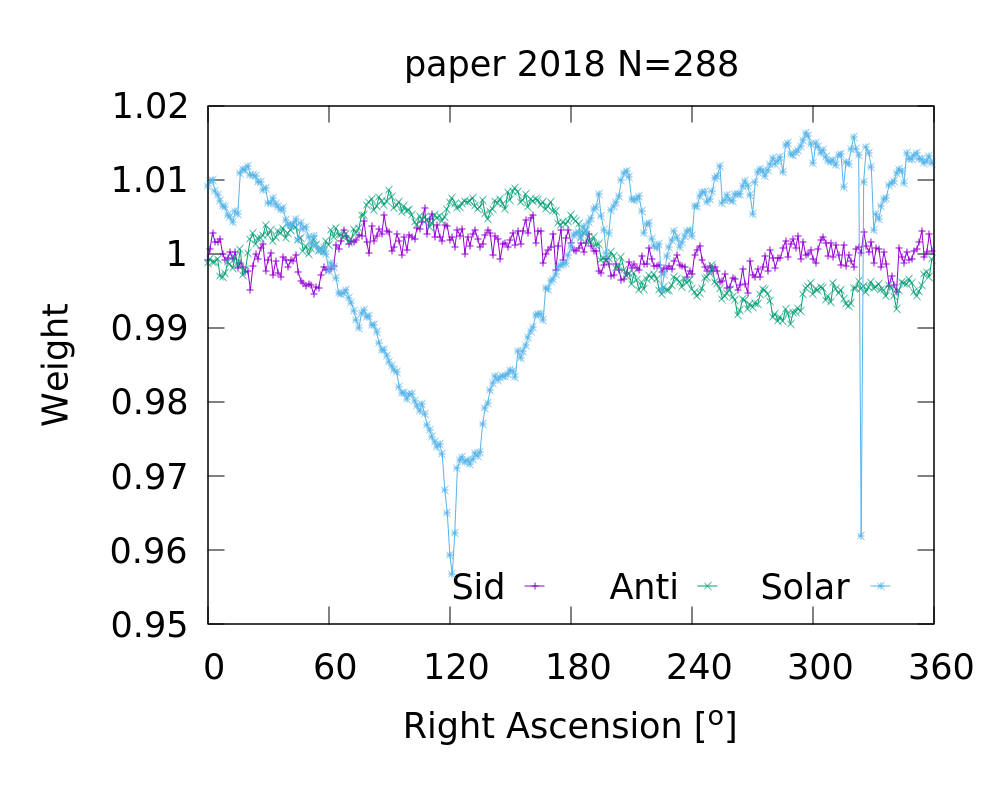
\includegraphics[width=\linewidth]{Graficos/solar_anti_sid_paper2018_in_288.png}
	\caption{Los pesos para las tres frecuencias tal como se calcula en el paper del 2018.}
	\label{fig:all_288_paper}
	\end{figure}


	\begin{figure}[H]
	\centering
	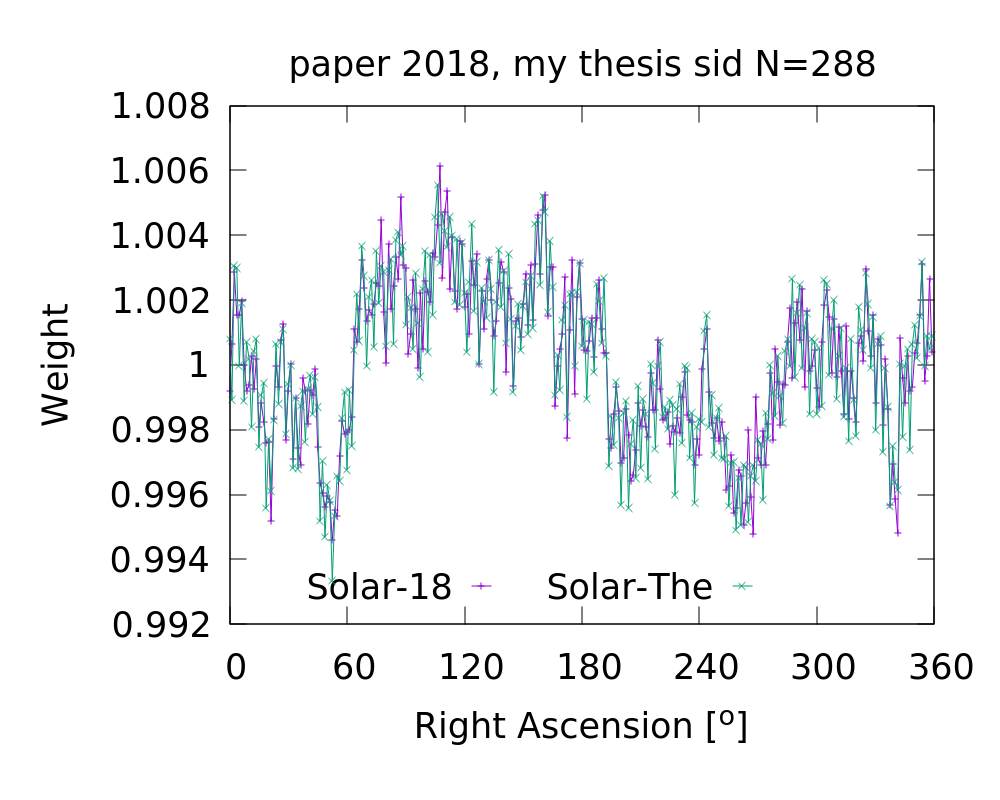
\includegraphics[width=\linewidth]{Graficos/sidereal_my_and_paper_in_288.png}
	\caption{Comparando los resultados del paper con mi código para la frecuencia sidérea para N=288}
	\label{fig:sidereal_288}
	\end{figure}


	Ya en la Fig.\,\ref{fig:sidereal_288}, se ve que la media de los pesos es algo razonable comparándolo con N=360, Fig.\ref{fig:solar_360}. Además que el error porcentual, usando como referencia los resultados del paper del 2018, es pequeña

	\begin{figure}[H]
	\centering
	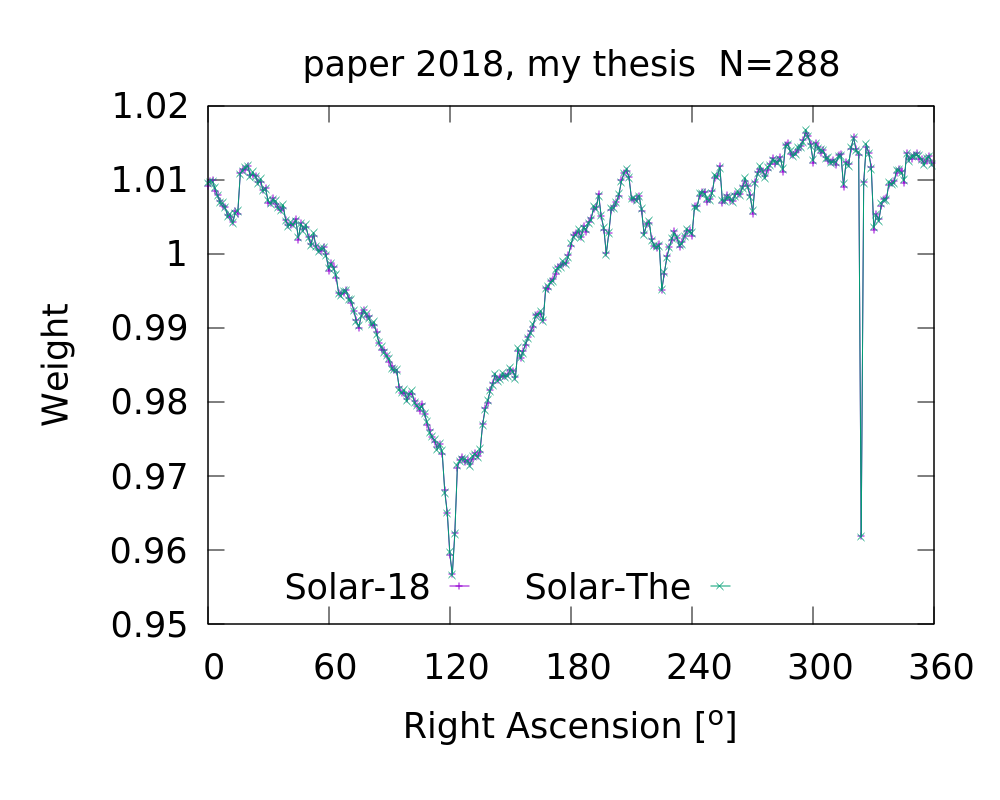
\includegraphics[width=\linewidth]{Graficos/solar_my_and_paper_2018_in_288.png}
	\caption{Pesos para la frecuencia solar.}
	\label{fig:solar_288}
	\end{figure}


	Para la frecuencia anti-sidérea no hay mucha diferencia a los obtenido para el caso de N=360. Los pesos se muestran en la Fig.\,\ref{fig:anti_288} 
	\begin{figure}[H]
	\centering
	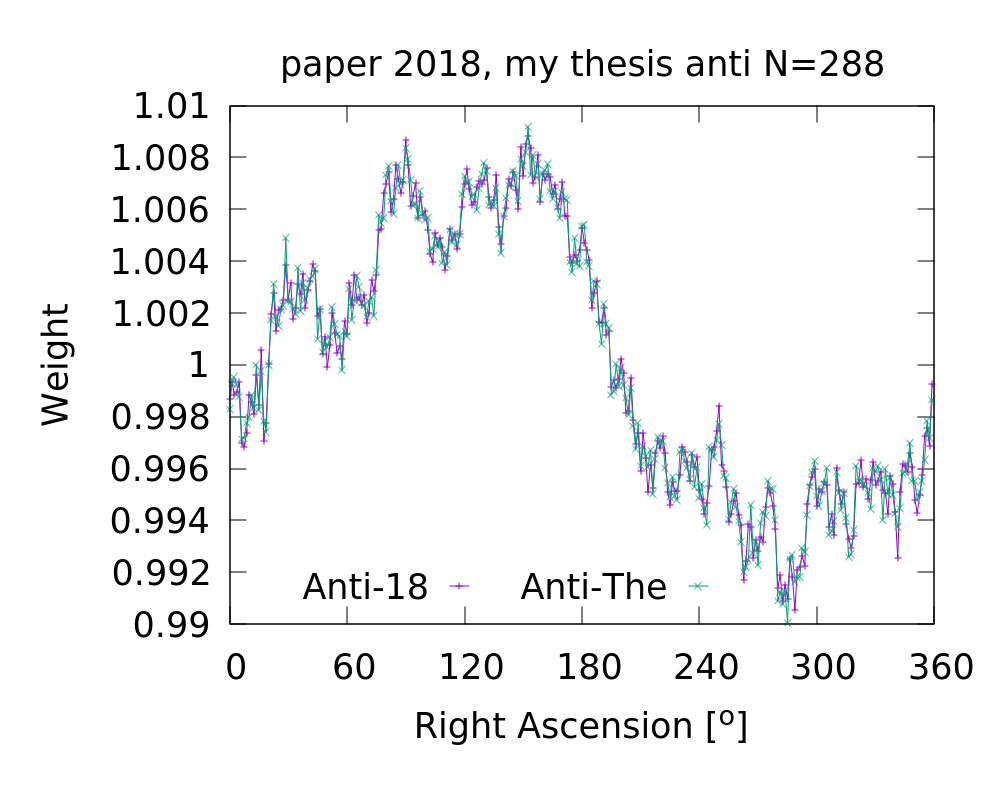
\includegraphics[width=\linewidth]{Graficos/anti_my_and_paper_2018_in_288.png}
	\caption{Pesos para la frecuencia anti-sidérea}
	\label{fig:anti_288}
	\end{figure}
